\chapter{Discussion}\label{ch:Discussion}


\section{GUI}
When a user of the system lay their eyes on the GUI, the first elements, they will see, are inputs for how many columns and rows should be in the grid that makes up the system as can be seen in \autoref{fig:GUI_screenshot_1}. Even though the user might be quite knowledgeable about networking, the will only be able to guess what this grid is. Therefore, an easy to implement solution could be to provide a simple description of the use case of the system. An even better solution could be to provide an image that changed along with the users input, and then provide some visualisation of the size of the grid such as axes to clarify even further that the user is changing the graph or grid that will make up the area where the devices in the network simulation can occupy.

\begin{figure}[H]
  \centering
  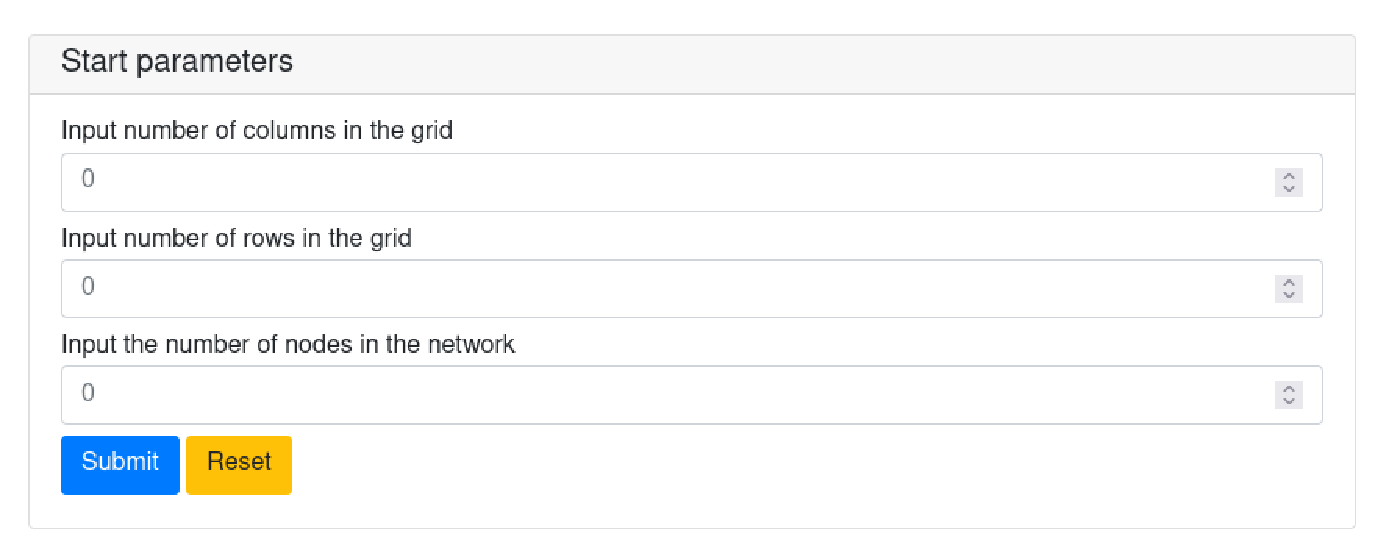
\includegraphics[width=0.9\textwidth]{GUI_screenshot_1.pdf}
  \caption{A screenshot of the first elements that are displayed when a user opens the GUI.}
  \label{fig:GUI_screenshot_1}
\end{figure}

\noindent Then, after the simulation has finished running, average metrics of the results from the individual nodes are displayed printed as is shown in \autoref{fig:GUI_screenshot_2}. An improvement to this implementation might incorporate an option to view the results from each individual node by either having the results in a simple table or implementing some way to display the results by having the user click on a button with the name of the node (i.e. Node n results). The option of using an element that is already present would be to enable the network topology graph to function as buttons, where the user would be able to click on the number of a given node and then have the results displayed. An example of the network topolgy graph can be seen in \autoref{fig:network_topology_example}.

\begin{figure}[h!]
  \centering
  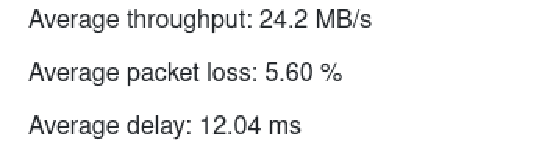
\includegraphics[width=0.5\textwidth]{GUI_screenshot_2.pdf}
  \caption{A screenshot of how the results of the simulation is outputted in GUI.}
  \label{fig:GUI_screenshot_2}
\end{figure}

\begin{figure}[h!]
  \centering
  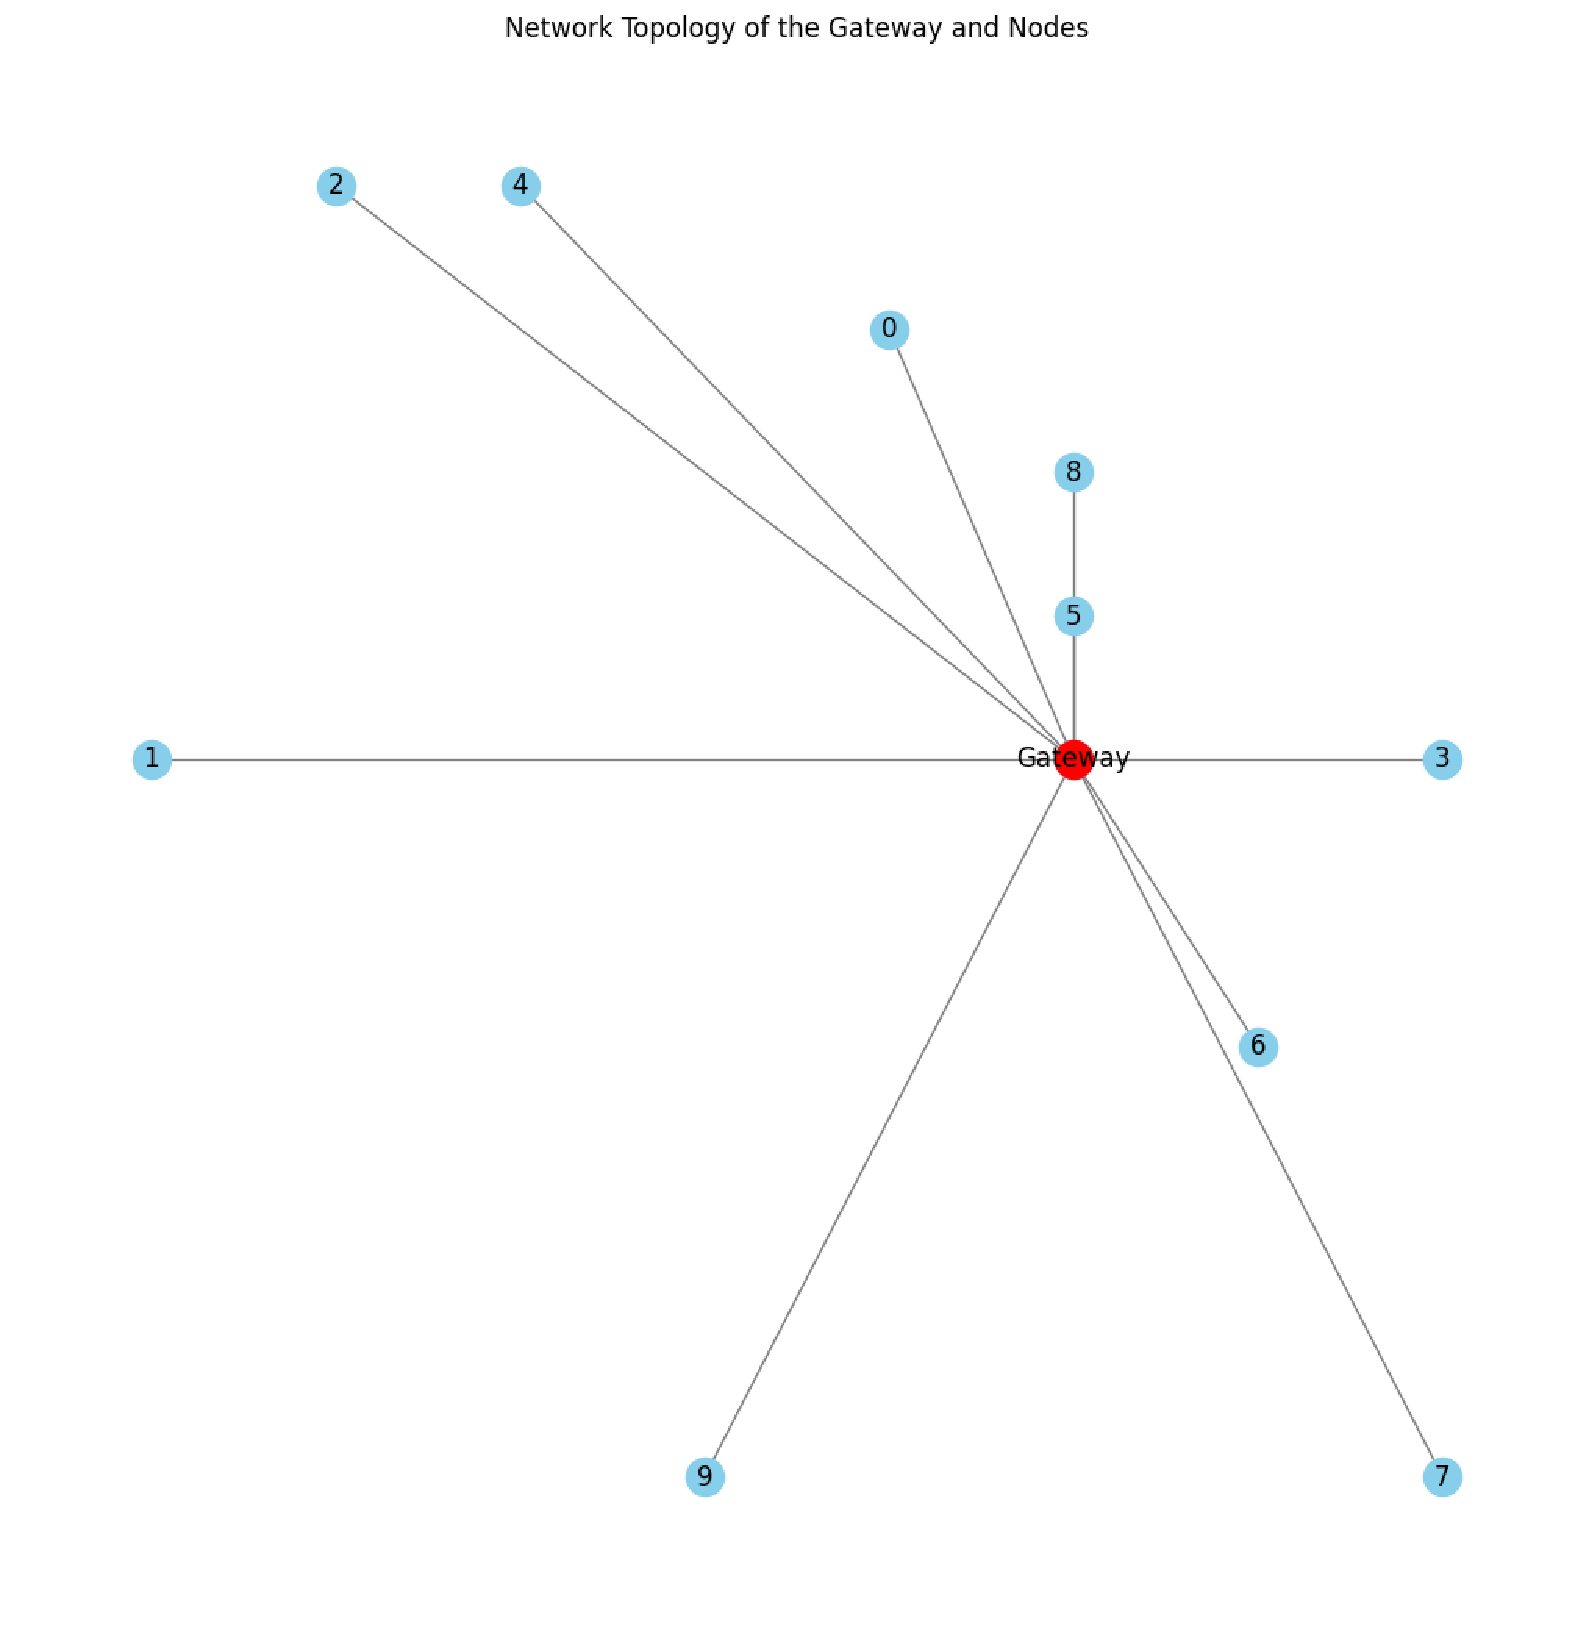
\includegraphics[width=0.6\textwidth, trim={2cm 2cm 2cm 2.5cm}, clip]{network_topology_example.pdf}
  \caption{A screenshot of how the network topology graph is outputted in the GUI.}
  \label{fig:network_topology_example}
\end{figure}


\section{Network}
As has already been described in \autoref{sec:Class_diagram_Network} and in the rest of \autoref{sec:Class_diagram}, a better implementation of how the system currently is implemented would have tried to get as close to functional cohesion as possible in order clarify and improve which object does what. As the implementation currently is, a name that more precisely describes the functionality of the \code{simulation} object would be \code{simulation\_and\_networking}. Of course, it must be acknowledged that complete functional cohesion will not make sense in this project, where the simulation will need to start the \code{network} after the positions of each \code{node} and \code{gateway} has been created.

\subsection{Network Performance Metrics}
Since the \code{network} is supposed to have as much cohesion as possible, it should also be able to store performance metrics independent of the \code{simulation}. In \autoref{fig:Class_diagram} the object \code{Network performance metrics} is set to have a dependency on the \code{network} object. In order to be true to this relationship between the two objects, \code{network} should be able to create the performance metrics and store them whether an instance of \code{simulation} exists or not. Therefore, \code{network} should check if \code{simulation} has an attribute in the \code{positions} list that belongs to a given node, that the \code{network} is going to store metrics about in the \code{Network performance metrics} object. This object could very well be some variant of an SQL database like PostgreSQL, MySQL, etc. It would also be possible to store the results of each simulation in some kind of NoSQL database like MongoDB or some kind if column-oriented database in order to have the organisation of the data resemble an SQL database.


\section{Device}
If the simulation had been implemented as an event based network simulator, where each event would take an amount of time that would then be summed after the simulation has finished, it would also make sense to enable instances of both the \code{node} and \code{gateway} objects to send and receive data over the network. Therefore, methods to send and receive data, should be included in the \code{device} object that then will be inherited by both the \code{node} and \code{gateway} objects. Along with these methods, there should also be attributes, where said data can be stored temporarily or maybe even until the simulation finishes.


\subsection{Node}
During the implementation, it was not necessary to implement some variant of threading or processes. However, if an actual event based simulator had been implemented, it would have made sense to make each instance of \code{node} and \code{gateway} have their own thread to allow them to still have access to the same resources. Though it might be necessary to split each instance into processes to make sure they do not overwrite each others attributes. Particularly in a scenario where a lot of nodes were instantiated, it would be beneficial to use threading or processes to make use of as much available computing power as possible to finish the simulation as fast as possible.


\subsection{Gateway}
As of the current implementation, the \code{gateway} is a subclass of both the \code{device} and \code{network}. One thing that this prevents, is that it only allows for one \code{gateway} to exist, if the methods and attributes of \code{network} are to be accessed through an instance of \code{gateway}. Therefore, \code{gateway} should only have been a subclass of \code{device}. It might also be preferable to make \code{gateway} able to report to \code{network} that a connection has been created or deleted, which would then change \code{connections} in accordance to the input from \code{gateway}.


\section{Simulation}
As can be seen in \autoref{fig:Class_diagram}, the \code{simulation} is the object that by far had most implemented methods and attributes. But no method to keep track of time or events was implemented. The method \code{add\_time} is then supposed to take an argument with how much time should be added to the total amount of elapsed time stored in the atribute \code{clock}. The idea of what unit of time should be used, was that it should just be an arbitrary unit based on integers in order to make it easier to implement on a computer. This would also enable the simulation to run faster instead of basing the duration of each event of the simulation on something like Pythons time library, where a start time would be recorded at the beginning of an event, which would then be subtracted from a timestamp recorded at the end of the given event.



































